%%%%%%%%%%%%%%%%%%%%%%%%%%%%%%%%%%%%%%%%%%%%%%%%%%%%%%%%%%%%%%%%
%% MS: Chasing Ecological Interactions.
%% Draft for PLoS Biology Research Matters blog
%% January 2016
%%%%%%%%%%%%%%%%%%%%%%%%%%%%%%%%%%%%%%%%%%%%%%%%%%%%%%%%%%%%%%%%
% Template for PLoS
% Version 3.1 February 2015
% % % % % % % % % % % % % % % % % % % % % %
% -- IMPORTANT NOTE
%
% This template contains comments intended 
% to minimize problems and delays during our production 
% process. Please follow the template instructions
% whenever possible.
% % % % % % % % % % % % % % % % % % % % % % % 
% Once your paper is accepted for publication, 
% PLEASE REMOVE ALL TRACKED CHANGES in this file and leave only
% the final text of your manuscript.
%
% There are no restrictions on package use within the LaTeX files except that 
% no packages listed in the template may be deleted.
%
% Please do not include colors or graphics in the text.
%
% Please do not create a heading level below \subsection. For 3rd level headings, use \paragraph{}.
% % % % % % % % % % % % % % % % % % % % % % %
%
% -- FIGURES AND TABLES
%
% Please include tables/figure captions directly after the paragraph where they are first cited in the text.
%
% DO NOT INCLUDE GRAPHICS IN YOUR MANUSCRIPT
% - Figures should be uploaded separately from your manuscript file. 
% - Figures generated using LaTeX should be extracted and removed from the PDF before submission. 
% - Figures containing multiple panels/subfigures must be combined into one image file before submission.
% For figure citations, please use "Fig." instead of "Figure".
% See http://www.plosone.org/static/figureGuidelines for PLOS figure guidelines.
%
% Tables should be cell-based and may not contain:
% - tabs/spacing/line breaks within cells to alter layout or alignment
% - vertically-merged cells (no tabular environments within tabular environments, do not use \multirow)
% - colors, shading, or graphic objects
% See http://www.plosone.org/static/figureGuidelines#tables for table guidelines.
%
% For tables that exceed the width of the text column, use the adjustwidth environment as illustrated in the example table in text below.
%
% % % % % % % % % % % % % % % % % % % % % % % %
%
% -- EQUATIONS, MATH SYMBOLS, SUBSCRIPTS, AND SUPERSCRIPTS
%
% IMPORTANT
% Below are a few tips to help format your equations and other special characters according to our specifications. For more tips to help reduce the possibility of formatting errors during conversion, please see our LaTeX guidelines at http://www.plosone.org/static/latexGuidelines
%
% Please be sure to include all portions of an equation in the math environment.
%
% Do not include text that is not math in the math environment. For example, CO2 will be CO\textsubscript{2}.
%
% Please add line breaks to long display equations when possible in order to fit size of the column. 
%
% For inline equations, please do not include punctuation (commas, etc) within the math environment unless this is part of the equation.
% % % % % % % % % % % % % % % % % % % % % % % %

\documentclass[10pt,letterpaper]{article}
\usepackage[top=0.85in,left=2.75in,footskip=0.75in]{geometry}

% Use adjustwidth environment to exceed column width (see example table in text)
\usepackage{changepage}

% Use Unicode characters when possible
\usepackage[utf8]{inputenc}

% textcomp package and marvosym package for additional characters
\usepackage{textcomp,marvosym}

% fixltx2e package for \textsubscript
\usepackage{fixltx2e}

% amsmath and amssymb packages, useful for mathematical formulas and symbols
\usepackage{amsmath,amssymb}

% cite package, to clean up citations in the main text. Do not remove.
\usepackage{cite}

% Use nameref to cite supporting information files (see Supporting Information section for more info)
\usepackage{nameref,hyperref}

% line numbers
\usepackage[right]{lineno}

% ligatures disabled
\usepackage{microtype}
\DisableLigatures[f]{encoding = *, family = * }

% rotating package for sideways tables
\usepackage{rotating}

% Remove comment for double spacing
%\usepackage{setspace} 
%\doublespacing
\usepackage{verbatim} % For comments - added by Pedro Jordano
% Text layout
\raggedright
\setlength{\parindent}{0.5cm}
\textwidth 5.25in 
\textheight 8.75in

% Bold the 'Figure #' in the caption and separate it from the title/caption with a period
% Captions will be left justified
\usepackage[aboveskip=1pt,labelfont=bf,labelsep=period,justification=raggedright,singlelinecheck=off]{caption}

% Use the PLoS provided BiBTeX style
\bibliographystyle{plos2015}

% Remove brackets from numbering in List of References
\makeatletter
\renewcommand{\@biblabel}[1]{\quad#1.}
\makeatother

% Leave date blank
\date{}

% Header and Footer with logo
\usepackage{lastpage,fancyhdr,graphicx}
\usepackage{epstopdf}
\pagestyle{myheadings}
\pagestyle{fancy}
\fancyhf{}
\lhead{\includegraphics[width=2.0in]{PLOS-submission.eps}}
\rfoot{\thepage/\pageref{LastPage}}
\renewcommand{\footrule}{\hrule height 2pt \vspace{2mm}}
\fancyheadoffset[L]{2.25in}
\fancyfootoffset[L]{2.25in}
\lfoot{\sf PLOS}

%% Include all macros below

\newcommand{\lorem}{{\bf LOREM}}
\newcommand{\ipsum}{{\bf IPSUM}}

%% END MACROS SECTION


\begin{document}
\vspace*{0.35in}

% Title must be 250 characters or less.
% Please capitalize all terms in the title except conjunctions, prepositions, and articles.
\begin{flushleft}
{\Large
\textbf{Chasing Ecological Interactions}
}
\newline
% Insert author names, affiliations and corresponding author email (do not include titles, positions, or degrees).
\\
\textbf{Pedro Jordano}\textsuperscript{1*,\Yinyang}
\\
\bigskip
\bf{1} Integrative Ecology Group, Estaci\'on Biol\'ogica de 
Do\~nana, CSIC, Pabell\'on del Per\'u, Avda. Mar\'ia Luisa, s/n, 
E-41013 Sevilla, Spain
\\
\bigskip

% Insert additional author notes using the symbols described below. Insert symbol callouts after author names as necessary.
% 
% Remove or comment out the author notes below if they aren't used.

% Use the asterisk to denote corresponding authorship and provide email address in note below.
* jordano@ebd.csic.es

\end{flushleft}
%
%%%%%%%%%%%%%%%%%%%%%%%%%%%%%%%%%%%%%%%%%%%%%%%%%%%%%%%% Abstract
% Keep the abstract below 100 words
\subsection*{Abstract}
% Please keep the Author Summary between 150 and 200 words
% Use first person. PLOS ONE authors please skip this step. 
% Author Summary not valid for PLOS ONE submissions.   
% 121 words -----------------------------------------------------
Basic research on Biodiversity has concentrated on the study of species, naming new species, studying distribution patterns, and analyzing their evolutionary relationships. Yet Biodiversity is more than a collection of individual species; it is the combination of biological entities and processes that supports the Earth system. Understanding Biodiversity requires its cataloguing, but also assessing the ways species interact with other species and provide a functional support for the Tree of Life. Ecological interactions may be lost well before the species interacting go extinct, so that their ecological functions disappear. Here I address the challenges in studying the functional aspects of species interactions and how basic research is helping us to address the current fast-paced extinction of species due to human activities.

\section*{Author Summary}
Biodiversity, all the different forms of life on Earth, is supported by ecological interactions among species. No single species on Earth lives without interacting with other species. Recent attempts to address the fast-paced loss of biodiversity are being supported by basic research stemming on its inventory (cataloguing species) but also in understanding how species are intertwined within complex webs of ecological interactions that support functional ecosystems.\\
\noindent\hrulefill
\bigskip
\linenumbers

%%%%%%%%%%%%%%%%%%%%%%%%%%%%%%%%%%%%%%%%%%%%%%%%%%%%%%%%%%%%%%%%%%
\begin{quotation}
  \textit{I am tempted to give one more instance showing how plants and animals, most remote in the scale of nature, are bound together by a web of complex relations}. (Darwin Ch. 1860. On the origin of species by means of natural selection. Chapter 3, p. 75).\\
  \textit{There is a much more insidious kind of extinction: the extinction of ecological interactions.}. (Janzen, D.H. 1974. The deflowering of Central America. Natural History, 83: 48-53).\\
\bigskip
\end{quotation}
%%%%%%%%%%%%%%%%%%%%%%%%%%%%%%%%%%%%%%%%%%%%%%%%%%%%%%%%%%%%%%%%%%
%\subsection*{Introduction}

Suppose you want to build the LEGO\circledR \textit{Triceratops Trapper} model (it is model no. 5885-1). It has 256 pieces, corresponding to 74 distinct parts. It's a relatively simple artifact; yet impossible to build by assembling these 256 pieces at random. To get the fully functional Triceratops Trapper we need to know not only the inventory of its parts: we also need to know how the different pieces are connected together. We'll have a functional Triceratops Trapper if and only if we assemble the model connecting its component pieces the right way. Species in ecosystems are not connected (linked) by random interactions; there are regularities independent on the type of ecosystem and even on the type of ecological interaction. This Web of Life \cite{Thompson:2009} defines the wireframe that supports Biodiversity, and ecological interactions provide essential services and functionality for its persistence. Interactions might be lost (extinct) even well before the species. For instance, the "empty forest syndrome" \cite{Redford:1992} describes situations where animals and plants may persist in disturbed areas (e.g,, a tropical forest fragment) yet with so much reduced abundances that their functional ecological role is lost. Interaction extinction may result in collapse of important ecological functions such as pollination and seed dispersal, crucial for forest regeneration and ecosystem persistence. These losses of interactions cause unprecedented changes in cascade in natural communities, implying losses of ecological functions that are crucial for ecosystem persistence. For example, just imagine the myriad consequences of extinctions of pollinators and frugivore seed dispersers for ecosystems like tropical rainforests, where more than 90\% of the woody plant species need their interactions to support their life cycles. 

Ecological interactions are the wireframe of biodiversity. No single species on Earth lives without interacting with other species. Thus, Biodiversity is more than just species: interactions among them are the architecture that supports ecosystems. It’s the Web of Life. Exploring and inventorying Biodiversity represents a fundamental challenge for basic research in ecology and conservation biology. This basic knowledge is urgently required to properly diagnose the status of Biodiversity conservation and develop early warning signals for situations of collapse. 

%-----------------------------------------------------------------
\subsection*{Diversity: of species and their interactions}

The Web of Life assembles species that interact with each other in a variety of ways, conforming complex interaction networks (Fig. 1). A myriad of interaction modes exists in nature and illustrates with fascinating details the complexity of natural histories of partner species. Forms of interaction include predation, competition, commensalism, amensalism, mutualism, symbiosis, parasitism and in all cases involve reciprocal effects for the interacting species. Recent basic research on the topology and structure of these networks has revealed universal patterns that ultimately affect their stability and resilience, yet we are far from fully documenting all the types of interaction modes that exist even in simple ecosystems. 

Just in the same way we sample individuals of free living species to estimate the diversity in a particular area or ecosystem, we can sample interactions. In this way we can assess the full complexity of ecosystem structure. Yet the exercise is not trivial. Because of their complexity, we are far from fully understanding the minimum set of functional links that are needed to support and restore damaged ecosystems.

Life on Earth is supported by zillions of interactions among species. Yet we lack robust estimates of the total number of species living on Earth, and even more we face the surmounting problem of assessing the diversity of their interactions; both are the main elements supporting the Web of Life. A complete understanding of these systems demands that a large fraction of these interactions be experimentally or computationally probed. This is very difficult, as rapid and effective actions or conservation and restoration of human-disturbed ecosystems urgently require the identification of the minimum amount of complexity that has to be restored in order to guarantee ecosystem’s persistence. 

Considering all the distinct ways in which such highly complex, interactive systems can be decomposed into parts cannot be done on a statistical basis (as, for example, with an ideal gas) because each interaction is particular; genomes, proteins, cells, and species interact in specific ways. The number of ways a complex system can be partitioned is known as Bell’s number $B_n$\cite{Koch:2012aa}. For three elements, there are $B_3 = 5$ such partitions; three species may not interact at all, or any two of them can interact, or all three, for a total of five possibilities. Understanding the system requires measuring the probability and magnitude of each of these five. This is out of the feasibility limits for any study\cite{Koch:2012aa}, given that Bell’s number scales supra-exponentially with the number of components. The number of actual pairwise interactions among species in local assemblages scales with species richness in real plant-animal webs (Fig. 1). These real ecological systems would be within the range of $n= 10^3-10^5$ or even $n= 10^4-10^{6.5}$ components, depending on spatial scale when we move from local to regional and up to continental spatial scales. To fully quantify the size of these interactomes we thus need to focus on what we know about the macroscopic properties of complex ecological interaction networks \cite{Thompson:2009}. 

\subsection*{Basic conservation science in the Anthropocene: challenges}
While the effects of the present biodiversity crisis have been largely focused on the loss of species, a missed component of biodiversity loss that often accompanies or even precedes species disappearance is the extinction of ecological interactions. A large body of evidence from field experimental ecology shows that cascading effects are most often triggered by species extinctions \cite{Dirzo:2014}. 

As vividly stated by Daniel H. Janzen, \textit{“What escapes the eye ... is a much more insidious kind of extinction: the extinction of ecological interactions”}. Loss of key ecological interactions may precede the local extinction of partner species that depend on the key ecological services provided. For example, a myriad of vertebrate species have experienced population declines and eventual extinctions matching human expansion, i.e. the “Anthropocene defaunation” \cite{Dirzo:2014}. Large bodied vertebrates have been especially hard hit, and as a result, many disturbed ecosystems currently host only small- to medium-bodied species. If the remnant, extant species fail to provide pivotal services formerly assisted by vanishing large vertebrates, human-driven defaunation may trigger negative cascading effects on ecosystem dynamics. This downgrading process is expected to result, for example, in collapsed mutualisms of pollination and seed dispersal for plants depending on them for regeneration.

Early signals of mutualism collapse may trigger severe population declines which lag behind the loss of seed dispersers or pollinators. Consider deforestation, logging, fragmentation and climate change, now evidenced to have significant impacts on tropical carbon stocks. An elusive and yet undetected change in carbon storage may be associated to the disruption of these mutualisms due to defaunation- the loss of animal pollinators and frugivores acting as seed dispersers- simply because forest regeneration may collapse.

\subsection*{Acknowledgments}
My work was funded by grant CGL2013-47429P and a Severo-Ochoa Excellence Grant (SEV2012-0262) from the Spanish Ministerio de Econom\'ia y Competitividad (MINECO), and RNM-5731 from the Junta de Andaluc\'ia. 

\nolinenumbers

%%%%%%%%%%%%%%%%%%%%%%%%%%%%%%%%%%%%%%%%%%%%%%%%%%%%%% References
\begin{thebibliography}{10}
\bibitem{Thompson:2009}
Thompson JN. The coevolving web of life. The American Naturalist 2009; 173: 125–140. doi:10.1086/595752

\bibitem{Redford:1992}
Redford KH. The empty forest. Bioscience. 1992; 42: 412–422. 

\bibitem{Dirzo:2014}
Dirzo R, Young HS, Galetti M, Ceballos G, Isaac NJB, Collen B. Defaunation in the Anthropocene. Science. 2014; 345: 401–406. doi: 10.1126/science.1251817

\bibitem{Lima-Mendez:2015}
Lima-Mendez G, Faust K, Henry N, Decelle J, Colin S, Carcillo F, et al. Ocean plankton. Determinants of community structure in the global plankton interactome. Science. 2015; 348: 1262073–1262073. doi:10.1126/science.1262073

\bibitem{Koch:2012aa}
Koch, C. Modular biological complexity. Science. 2012; 337: 531–532. doi:10.1126/science.1218616

\end{thebibliography}

%%%%%%%%%%%%%%%%%%%%%%%%%%%%%%%%%%%%%%%%%%%%%%%%%%%%%%%%% FIGURES
%------------------------------------------------------- Figure 1
\begin{figure}[h]
\begin{adjustwidth}{-2.25in}{0in}
\caption{\textbf{The structure of ecological interactions}. Top, examples of ecological interactions between plants and animals. a, \textit{Ramphastos vitellinus} feeding on \textit{Euterpe edulis} (Arecaceae) fruits; b; \textit{Ectatomma tuberculatum} over extra-floral nectaries at the base of a leaf of \textit{Qualea multiflora} (Vochysiaceae); c, \textit{Xylocopa violacea} visiting a flower of \textit{Allium} sp. (Amaryllidaceae). Bottom, different visualizations of the complexity of interaction networks among species (colored spheres) illustrated by their actual links (light grey lines): d, food webs typically describe all the interactions occurring in a given ecosystem with multiple trophic levels; e, most plant–animal interactions can be displayed as bipartite graphs describing the pairwise pattern of mutual interdependencies among two distinct sets of animals (orange nodes) and plants (yellow); f, interactions among species with a higher degree of intimacy, such as ant-plants show a distinct pattern of structure, often with multiple distinct groups (modules) of closely intimate associations. Photos: \copyright Guto Baileiro, with permission, \copyright Kleber del-Claro, with permission; and Pedro Jordano. Images d, e, and c produced with FoodWeb3D, written by R.J. Williams and provided by the Pacific Ecoinformatics and Computational Ecology Lab (www.foodwebs.org).}
\label{fig1}
  \begin{center}
    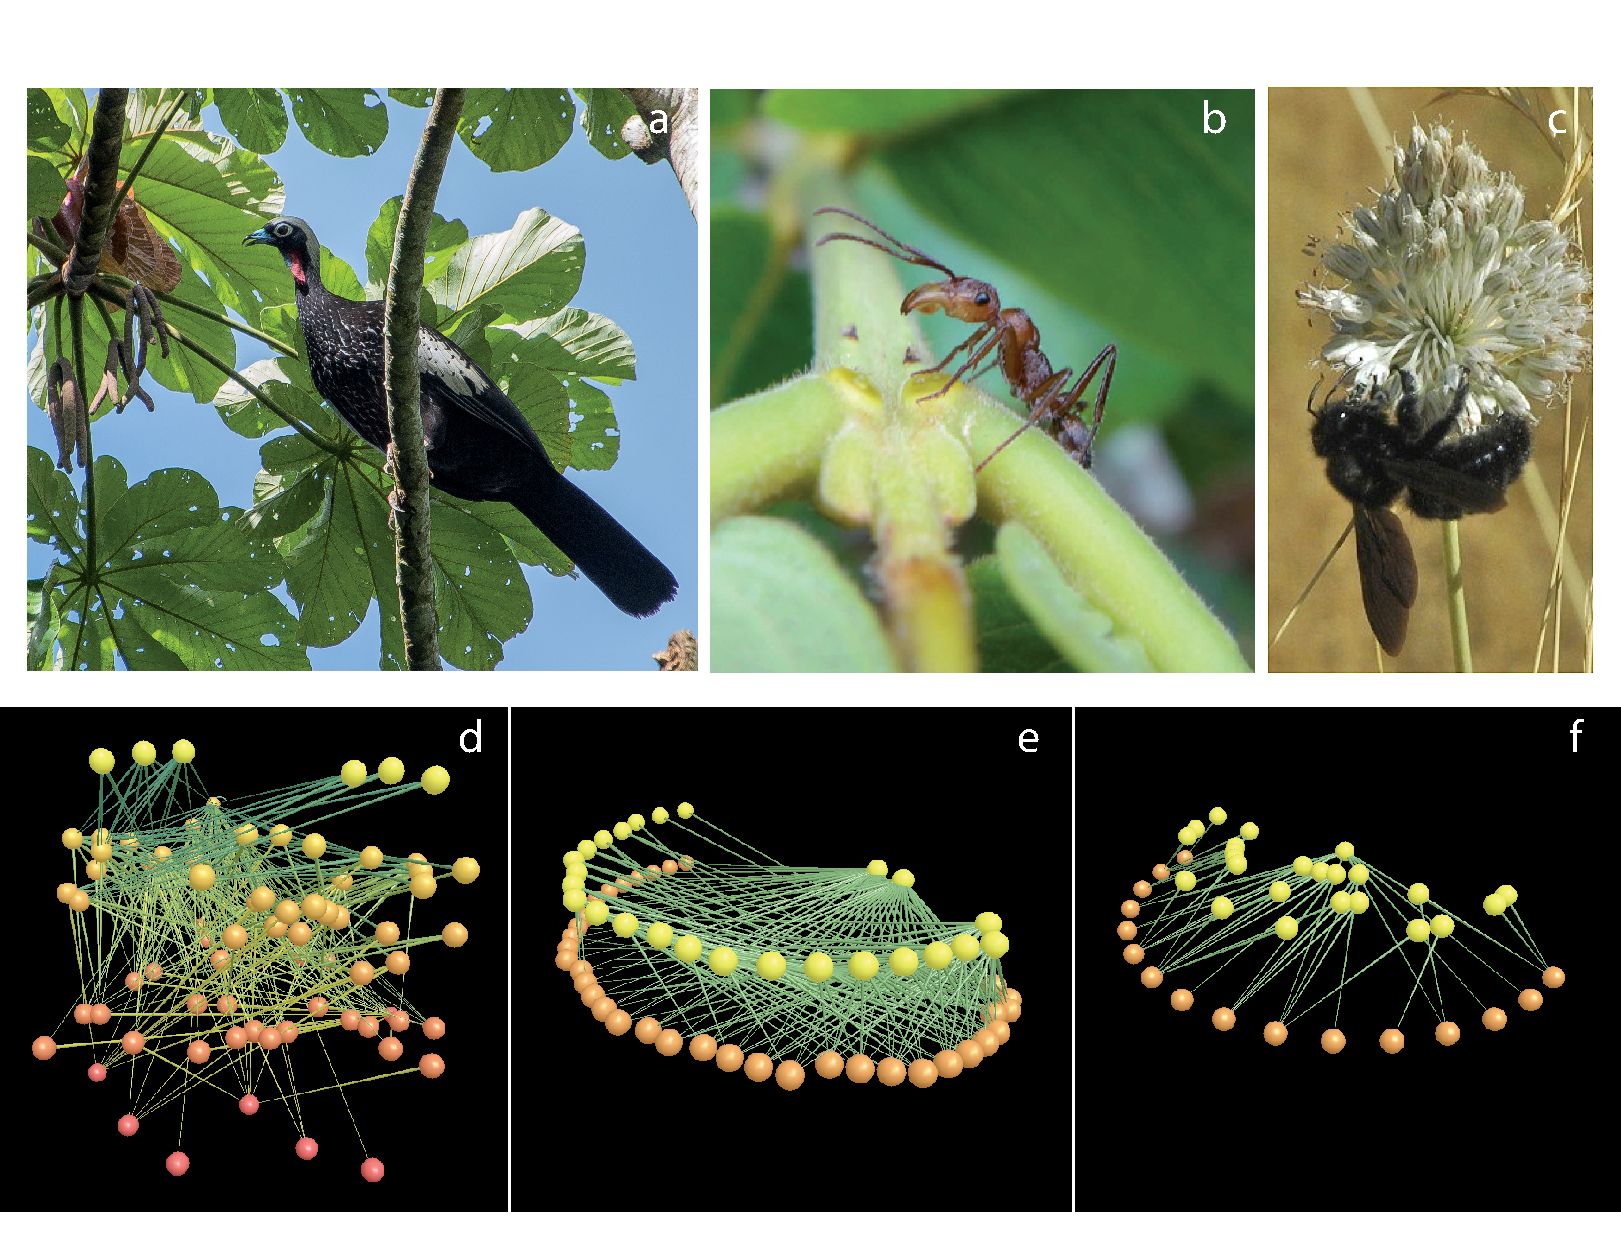
\includegraphics[width=17cm]{Fig1.pdf}
  \end{center}
\end{adjustwidth}
\end{figure}
%%%%%%%%%%%%%%%%%%%%%%%%%%%%%%%%%%%%%%%%%%%%%%%%%%%%%%%% MS NOTES
\begin{comment}
Organization of the Manuscript:

· Title: fewer than 75 characters\\
· Abstract: \ensuremath{\sim} 100 words\\
· Readers decide whether to read an article on the basis of the title and abstract – so, it is essential to get these right. Aim for a title that is clear, concise, and stimulates the general reader’s interest. Your abstract should be brief and explain in accessible language the key message of your article.\\
· Length: 800--1,000 words. There are no strict length limits, but in general Research Matters are very brief.\\
· References: \ensuremath{\sim}10. There are no strict reference limits, but in general Research Matters contain very few, necessary references. PLOS uses the numbered citation method, with references listed in numerical order of appearance.\\
%
%\section*{References}
% Either type in your references using
% \begin{thebibliography}{}
% \bibitem{}
% Text
% \end{thebibliography}
%
% OR
%
% Compile your BiBTeX database using our plos2015.bst
% style file and paste the contents of your .bbl file
% here.
% 
· Display items (images\slash figures, text boxes, tables): 1. Figures\slash images must be published under our Creative Commons Attribution License (CC BY), thus, in general, we cannot re-use previously published work. Please ensure that your submitted figure is in either .EPS or .TIFF format and of high enough resolution (at least 300dpi).

\end{comment}

\end{document}

